\chapter{Counterfactual Reasoning}
\label{ch-counterf}
This chapter is mostly based on 
Ref.\cite{pearl-2019review}, a 2019
 review of causality by Pearl.

This chapter
assumes that the reader
has read
Chapter \ref{ch-do-calc}
on do-calculus and
Chapter \ref{ch-linear-sys}  
on LDEN (linear 
deterministic systems
with external noise).

\section*{The 3 Rungs of Causal AI}
According to 
Judea Pearl,
there are 3 rungs in the
ladder of causal AI.
These are (as I see them):
\begin{enumerate}
\item
{\bf Observing Dumbly:} Collecting 
data
and fitting curves to it,
without any plan 
designed to
investigate Nature's 
causal connections.
\item {\bf Doing causal
experiments:} 
Doing experiments 
consciously designed to
elucidate
Nature's causal connections.
Even cats do this!, but current AI doesn't.
\item {\bf Imagining
 counterfactual situations, Analogizing:}
Imagining gedanken experiments
to further understand
Nature's causal connections,
and to decide what future
courses of action are
more likely to succeed,
even if there is zero
direct data for 
those courses of action.
Making
predictions based
on zero direct data is a very Bayesian
concern, well out of the purview of 
frequentists. Nevertheless,
humans do such
``analogizing" 
all the time to great advantage.
It becomes
possible if there
is some indirect but similar
data that can be transported
(transplanted, applied)
to the situation of
interest.
\end{enumerate}
Chapter \ref{ch-mp}
on message passing
is about rung 1.
Chapter \ref{ch-do-calc}
on do-calculus is about rung 2.
This chapter is dedicated to rung 3.



\section*{Two kinds of
 intervention operators}
In Chapter \ref{ch-do-calc},
we introduced a {\bf do operator}
$\rho_{\rvx=x}$ (
this is our notation for what Pearl 
symbolizes by $do(\rvx)=x$).
The study of counterfactuals 
requires that we
introduce a new
kind of intervention
operator that we will
call an {\bf imagine operator}
and denote by $\kappa_{\rvx\rarrow\rva}(x)$.

The 2  types of
intervention operators
are defined 
graphically in Fig.\ref{fig-rho-kappa}.
\begin{itemize}
\item
The do operator $\rho_{\rvx=5}$
(called $\rho$ because  it turns $\rvx$
into a root node)
amputates
the incoming arrows of node $\rvx$
and sets the TPM
of the new root node $\rvx$
to a delta function $\delta(x, 5)$
(or some state of $\rvx$ other than 5).
Sometimes it is convenient,
rather than calling the
new node $\rvx$ like
the old one, to call
it by the new name $\rho\rvx$.
\item
The imagine operator 
$\kappa_{\rvx\rarrow\rvb}(5)$
(called $\kappa$ because it
 creates konstant nodes)
operates on arrows
unlike the 
$\rho$ operator which operates on nodes.
$\kappa_{\rvx\rarrow\rvb}(5)$
deletes
arrow $\rvx\rarrow\rvb$
and
creates a new root node 
$\rvx'$
and a new arrow
$\rvx'\rarrow \rvb$. The
TPM of the new node $\rvx'$ is a 
delta function $\delta(x', 5)$
(or some state of $\rvx$ other than 5).
Sometimes it is convenient,
rather than calling the
new node $\rvx'$, to call
it by the 
more
explicit name $\kappa_\rvb\rvx$.
\end{itemize}

Now that we have 
both a do and an imagine operator,
we realize,
as Pearl did long ago,
that we can create
a {\bf do-imagine-calculus}
whose
objective
is to 
express
probabilities such as 
$P(\rvy|\rho\rvr=r, 
\kappa_\rvb \rvs=s, t)$
in terms of observable 
probabilities
that do not
contain
any do or imagine
operators in them.
As with
do-calculus,
this reduction
is not 
always possible,
and we say a probability is
{\bf identifiable}
if it  can be reduced
in that manner.
Such a do-imagine-calculus
has already
been developed
by Pearl and collaborators,
but
we won't 
discuss it in this chapter (perhaps
we  will discuss it
in a future one).


\begin{figure}[h!]
\centering
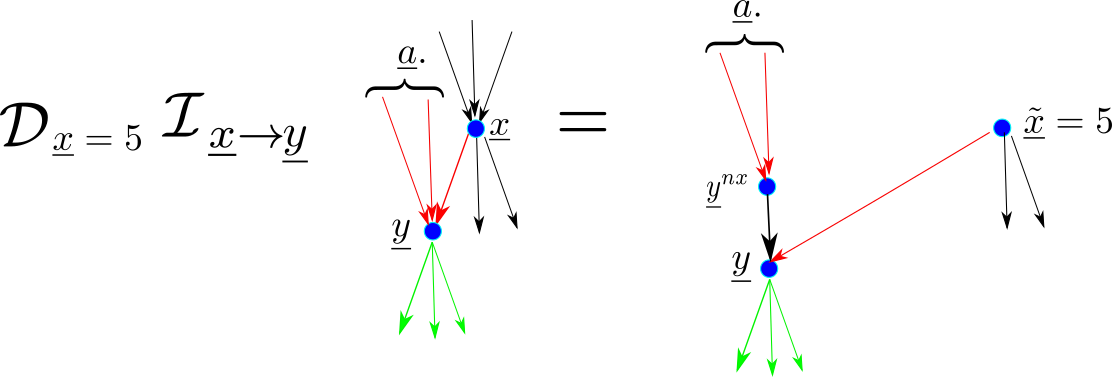
\includegraphics[width=3.5in]
{counterf/rho-kappa.png}
\caption{Action
of ``do" operator $\rho_{\rvx=5}$
on node $\rvx$
and of ``imagine" operator 
$\kappa_{\rvx\rarrow \rvb}(5)$
on arrow $\rvx\rarrow \rvb$.} 
\label{fig-rho-kappa}
\end{figure}


\section*{Do operator
$\rho_{\rva=a}$  for DEN diagrams}
By the end of
this chapter,
the two kinds of
intervention operators
will be applied to
DEN diagrams.
Let us begin that 
journey
by showing 
in this section
how
to apply  
the already familiar
do operator to
DEN diagrams.

Recall that
the structural
equations
for a linear DEN, as
given
by Eq.(\ref{eq-mat-fully-conn})
of Chapter \ref{ch-linear-sys}, are:

\beq
\rvx=A\rvx +\rvu
\;.
\label{eq-struc-pre-rho}
\eeq
Therefore,

\beq
\rvx=(1-A)^{-1}\rvu
\eeq
which
can be 
represented for
both linear
and non-linear DEN
diagrams by:

\beq
\rvx_i = x_i(\rvu.)
\eeq 

If now
we apply the
operator
$\rho_{\rva=a}$
to 
the diagram
described by
the structural
equations Eqs.\ref{eq-struc-pre-rho},
we get the following
new
structural
equations:

\beq
\rvx^*_i =\left\{
\begin{array}{lll}
 \sum_{j<i} A_{i|j}\rvx^*_j + \rvu_i&
 \text{if $\rvx_i\neq \rva$}
\\
a&
\text{if $\rvx_i=\rva$}
\end{array}
\right.
\label{eq-ith-struc-post-rho}
\;,
\eeq
where we are
calling 
$\rvx^*_i$ the
nodes
of the DEN 
diagram post intervention.

Eqs.(\ref{eq-ith-struc-post-rho})
can be expressed in matrix notation
as follows.
Define $\pi_\rva$ to
be the $nx\times nx$ matrix 
with all entries equal
to  zero
except for the $(i_0,i_0)$ entry, which is 1.
And define $e_\rva$
to be the column vector
with all entries zero
except for the $i_0$'th one, 
which is 1. 
Here
$i_0$  
is
defined so that $\rvx_{i_0}=\rva$.
In other words, $\pi_\rva$ and $e_\rva$
are defined by

\beq
(\pi_\rva)_{i,j}= \indi(i=j, \rva=\rvx_i)
\;
\eeq
and

\beq
(e_\rva)_i=\indi(\rva=\rvx_i)
\;,
\eeq
for $i, j\in \{0, 1, \ldots, nx-1\}$.
Next define

\beq
\pi_{!\rva}=1-\pi_\rva
\;,
\eeq

\beq
A^*=\pi_{!\rva} A
\;,
\eeq
and

\beq
\rvu_{!\rva}=\pi_{!\rva} \rvu
\;.
\eeq
The effect
of pre-multiplying
the matrix
$A$ 
and the column vector $\rvu$ by
$\pi_{!\rva}$
is to leave all rows
intact except for
the $i_0$
row, which is set to zero. Here
 $i_0$ is defined by
 $\rva=\rvx_{i_0}$.
Finally,
using 
all
of the
variables just defined,
we can express the
structural equations
of the linear DEN diagram,
post intervention, as


\beq
\rvx^*= A^* \rvx^* + \rvu_{!\rva} +
ae_\rva
\;.
\eeq
Thus,

\beq
\rvx^*=(1-A^*)^{-1} (\rvu_{!\rva}+ae_\rva)
\;.
\eeq
which
can be 
represented for
both linear
and non-linear DEN
diagrams by:

\beq
\rvx^*_i=x^*_i(\rvu_{!\rva},a)
\;.
\eeq



For any bnet,

\beq
P(\rvy=y|\rvx=x)
=
P_{G}(\rvy=y|\rvx=x)
\eeq

\beq
P(\rvy=y|\rho\rvx=x)
=
P_{\rho_{\rvx=x}G}(\rvy=y)
\eeq


\begin{claim}
For a non-linear DEN diagram,



\beq
P(y|\rho\rvx=x)=
E\left[
\delta[y, y(\rvu_{!\rvx},x)]\right]
\;.
\eeq
\end{claim}
\proof
\beqa
P(\rvy=y|\rho\rvx=x)
&=&
P_{\rho_{\rvx=x}G}(\rvy=y)
\\
&=&\sum_{u_{!\rvx}}P(u_{!\rvx})
P_{\rho_{\rvx=x}G}
(\rvy=y|u_{!\rvx})
\\
&=&\sum_{u_{!\rvx}}P(u_{!\rvx})
\delta[y, y(u_{!\rvx},x)]
\\
&=&
E_{\rvu_{!\rvx}}
[\delta[y, y(u_{!\rvx}, x)]]
\\
&=&
E[\delta[y,y(\rvu_{!\rvx}, x)]]
\eeqa
\qed

\begin{claim}
For a nonlinear DEN diagram,

\beq
E[\rvy|\rho \rvx=x]=
E[y(\rvu_{!\rvx}, x)]
\;.
\eeq
\end{claim}
\proof

\beqa
E[\rvy|\rho \rvx=x]
&=&
\sum_{y}
yP(\rvy=y|\rho\rvx=x)
\\
&=&
\sum_{y}
yE[
\delta[y, y(u_{!\rvx},x)]]
\\
&=&
E[y(\rvu_{!\rvx}, x)]
\eeqa
\qed


For any bnet
\beqa
P(y|\rho\rvx=x, z)&=&
\frac{P(y, z|\rho\rvx=x)}
{P(z|\rho\rvx=x)}
=
P_{\rho_{\rvx=x}G}(y|x, z)
\eeqa

For a nonlinear DEN diagram,
\beq
P(y, z|\rho\rvx=x)
=
\sum_{u_{!\rvx}}P(u_{!\rvx})
\delta[y, y(u_{!\rvx},x)]
\delta[z, z(u_{!\rvx},x)]
\eeq

\beq
P(z|\rho\rvx=x)=
\sum_{u_{!\rvx}}P(u_{!\rvx})
\delta[z, z(u_{!\rvx},x)]
\;.
\eeq

\section*{Mediation Analysis}
In
the previous section,
we applied the do operator 
to DEN diagrams.
Mediation analysis
is a nice example
which applies
both
do and 
imagine operators
to DEN diagrams.


\begin{figure}[h!]
$$\xymatrix{
\rvu_\rvt\ar[dd]
&\rvu_\rvm\ar[d]
&\rvu_\rvy\ar[dd]
\\
&\rvm\ar[rd]
\\
\rvt\ar[ru]\ar[rr]&&\rvy
\\
&G
}
\;\;\;\;\;\;\;\;\;\;\;\;
\xymatrix{
\rvu_\rvt\ar[dd]\ar@/^2pc/@{<-->}[r]
&\rvu_\rvm\ar[d]\ar@/^2pc/@{<-->}[r]
&\rvu_\rvy\ar[dd]
\\
&\rvm\ar[rd]
\\
\rvt\ar[ru]\ar[rr]&&\rvy
\\
&G^*
}$$
\caption{Graphs $G$ and $G^*$
are used to 
discuss mediation.
In graph
$G$,
the exogenous
variables are independent,
whereas in graph $G^*$
they are not.}
\label{fig-mediation-bnets}
\end{figure}

The term ``mediation analysis"
refers
to  the analysis
of the DEN diagram
$G$
in Fig.\ref{fig-mediation-bnets}.
In that diagram,
node $\rvt$ 
influences node
$\rvy$
both
directly
and via the mediator node $\rvm$.
The structural 
equations for that diagram
are of the form:

\begin{subequations}
\label{eq-struc-eqs-med}
\beqa
\rvt&=&\rvu_\rvt
\\
\rvm&=&f_\rvm(\rvt, \rvu_\rvm)
\\
\rvy&=&f_\rvy(\rvt, \rvm, \rvu_\rvy)
\;.
\eeqa
\end{subequations}
Thus,

\beq
\rvy=f_\rvy(u_\rvt, 
f_\rvm(\rvu_\rvt, \rvu_\rvm), \rvu_\rvy)
\;.
\eeq

\begin{figure}[h!]
\centering
\begin{tabular}{m{6cm}m{6cm}}
$\xymatrix{
\rvu_\rvt
&\rvu_\rvm\ar[d]
&\rvu_\rvy\ar[dd]
\\
&\rvm\ar[rd]
\\
\rvt=5\ar[ru]
\ar[rr]&&\rvy
}$
&
$\xymatrix{
\rvu_\rvt\ar[dd]
&\rvu_\rvm\ar[d]
&\rvu_\rvy\ar[dd]
\\
&\rvm\ar[rd]
\\
\rvt\ar[ru]^{\kappa(5)}
\ar[rr]
&&\rvy
}$
\\
\\
$\;\;\;\;\;\;\;\;
\rho_{\rvt=5}G$
&
$\;\;\;\;\;\;\;\;
\kappa_{\rvt\rarrow\rvm}(5)G$
\end{tabular}
\caption{Graph $G$
of Fig.\ref{fig-mediation-bnets}
after applying do operator $\rho_{\rvt=5}$
and imagine operator 
$\kappa_{\rvt\rarrow\rvm}(5)$.}
\label{fig-mediation-ops-egs}
\end{figure}

If we apply
$\rho_{\rvt=5}G$
to Eqs.(\ref{eq-struc-eqs-med}), we get

\begin{subequations}
\label{eq-mediation-rho-egs}
\beqa
\rvt&=&5
\\
\rvm&=&f_\rvm(\rvt, \rvu_\rvm)
\\
\rvy&=&f_\rvy(\rvt, \rvm, \rvu_\rvy)
\;.
\eeqa
\end{subequations}
Eqs.\ref{eq-mediation-rho-egs}
are represented graphically
in Fig.\ref{fig-mediation-ops-egs}.
We will often denote the  random variable
 $\rvy$ in Eqs.(\ref{eq-mediation-rho-egs})
by the more explicit symbol 
$\rvy_{\rho_{\rvt=5}G}$.
Pearl often 
refers to
this $\rvy$ by the less explicit symbol
$Y_5$ or $Y_5(u)$ where $Y=\rvy$
and $u=(u_\rvm, u_\rvy)=u_{!\rvt}$.

If we apply
$\kappa_{\rvt\rarrow\rvm}(5)G$
to Eqs.(\ref{eq-struc-eqs-med}), we get

\begin{subequations}
\label{eq-mediation-kappa-egs}
\beqa
\rvt&=&\rvu_\rvt
\\
\rvm&=&f_\rvm(5, \rvu_\rvm)
\\
\rvy&=&f_\rvy(\rvt, \rvm, \rvu_\rvy)
\;.
\eeqa
\end{subequations}
Eqs.\ref{eq-mediation-kappa-egs}
are represented graphically
in Fig.\ref{fig-mediation-ops-egs}.
We will often denote the  random variable
 $\rvy$ in Eqs.(\ref{eq-mediation-kappa-egs})
by the more explicit symbol 
$\rvy_{\kappa_{\rvt\rarrow\rvm}(5)G}$.
 Pearl often 
refers to
this $\rvy$ by the less explicit symbol
$Y_5$ or $Y_5(u)$ where $Y=\rvy$
and $u=(u_\rvt, u_\rvm, u_\rvy)$.

\hrule

\begin{figure}[h!]
\centering
\begin{tabular}{m{6cm}m{6cm}}
$
\xymatrix{
\rvu_\rvt
&\rvu_\rvm\ar[d]
&\rvu_\rvy\ar[dd]
\\
&\rvm\ar[rd]
\\
\rvt=t\ar[ru]
\ar[rr]&&\rvy
}$
&
$
\xymatrix{
\rvu_\rvt
&\rvu_\rvm
&\rvu_\rvy\ar[dd]
\\
&\rvm=m\ar[rd]
\\
\rvt=t
\ar[rr]&&\rvy
}$
\\
\\
$\;\;\;\;\;\;\;\;
\rho_{\rvt=t}G$
&
$\;\;\;\;\;\;\;\;
\rho_{\rvt=t}\rho_{\rvm=m}G$
\end{tabular}
\caption{Graph $G$
of Fig.\ref{fig-mediation-bnets}
after applying the 
do operators $\rho_{\rvt=t}$
and
$\rho_{\rvt=t}\rho_{\rvm=m}$.}
\label{fig-mediation-rho}
\end{figure}
Define the Total Effect (TE),
and the
Controlled Direct Effect (CDE) by
\beqa
TE&=& E[
\rvy_{\rho_{\rvt=1}G}
-\rvy_{\rho_{\rvt=0}G}
]
\\
CDE(m)&=&
E[
\rvy_{\rho_{\rvt=1}\rho_{\rvm=m}G}
-\rvy_{\rho_{\rvt=0}\rho_{ \rvm=m}G}
]
\eeqa
The two DEN diagrams
$\rho_{\rvt=t}G$
and
$\rho_{\rvt=t}\rho_{\rvm=m}G$
used in the definitions
of $TE$ and $CDE$
are given in Fig.\ref{fig-mediation-rho}.
\hrule

\begin{figure}[h!]
\centering
\begin{tabular}{m{4cm}m{3cm}}
$
\kappa_{\rvt\rarrow\rvy}(a)
\kappa_{\rvt\rarrow\rvm}(b)G
=$
&
$\xymatrix{
\rvu_\rvt\ar[dd]
&\rvu_\rvm\ar[d]
&\rvu_\rvy\ar[dd]
\\
&\rvm\ar[rd]
\\
\rvt\ar[ru]^{\kappa(b)}
\ar[rr]^{\kappa(a)}&&\rvy
}$
\end{tabular}
\caption{
Graph $G$
of Fig.\ref{fig-mediation-bnets}
after
applying the 
imagine operator
 $\kappa$
 to arrows
$\rvt\rarrow\rvm$ and $\rvt\rarrow\rvy$.}
\label{fig-mediation-kappa}
\end{figure}

Let

\beq
\caly^b_a=
 E[
\rvy_{\kappa_{\rvt\rarrow\rvy}(a)
\kappa_{\rvt\rarrow\rvm}(b)G}
]
\eeq
Fig.\ref{fig-mediation-kappa}
shows the diagram 
$\kappa_{\rvt\rarrow\rvy}(a)
\kappa_{\rvt\rarrow\rvm}(b)G$
used in
the definition of $\caly^b_a$.


Now define the
Natural Direct Effect (NDE), and the
Natural Indirect Effect (NIE)
by
\beqa
NDE
&=&\caly_1^0 - \caly_0^0
\\
NIE(t)
&=&\caly_t^1 - \caly_t^0
\;.
\eeqa

Note that
\beqa
NDE+NIE(1)&=&(\caly_1^0-\caly_0^0)+(\caly_1^1 - \caly_1^0)
\\
&=&\caly_1^1-\caly_0^0
\\
&=&
TE
\;.
\eeqa


